\documentclass[a4paper,10pt]{report}
\usepackage{Cours}
\usepackage{delarray}
\usepackage{fancybox}
\newcommand{\Sum}[2]{\ensuremath{\textstyle{\sum\limits_{#1}^{#2}}}}
\newcommand{\Int}[2]{\ensuremath{\mathchoice%
	{{\displaystyle\int_{#1}^{#2}}}
	{{\displaystyle\int_{#1}^{#2}}}
	{\int_{#1}^{#2}}
	{\int_{#1}^{#2}}
	}}
\usepackage{pstricks-add}



\begin{document}
% \everymath{\displaystyle}

\maketitle{Chapitre 12}{Espaces vectoriels normés}

Dans tout ce chapitre, $E$ désigne un $\mathbb{K}$-espace vectoriel de \emph{dimension finie} avec $\mathbb{K}= \mathbb{R}$ ou $\mathbb{C}$. La valeur absolue (ou le module selon le cas) d'un réel (ou d'un complexe) $x$, sera noté $\vert x \vert$.

 \section{Espaces vectoriels normés}
 
 Dans cette section, $E$ n'est pas nécessairement de dimension finie.
 
 \subsection{Normes}
 
 \begin{Definition}{} On appelle \emph{norme} sur $E$ toute application $N : E \rightarrow \mathbb{R}_+$ vérifiant les propriétés suivantes :
 
 \begin{itemize}
 \item \emph{Homogénéité} :
 
% Pour tout $\lambda \in \mathbb{K}$ et pour tout $x \in E$, $N(\lambda x) = \vert \lambda \vert N(x)$ (\emph{homogénéité}).
 \item \emph{Séparation} :
 
% Pour tout $x \in E$, $N(x)=0$ si et seulement si $x=0_E$ (\emph{séparation}).
 \item \emph{Inégalité triangulaire} :
 
% Pour tout $(x,y) \in E^2$, $N(x+y) \leq N(x)+ N(y)$ (\emph{inégalité triangulaire}).
 \end{itemize}
 
Le couple $(E,N)$ est alors appelé \emph{espace vectoriel normé}. On peut ne pas préciser la norme si il n'y a pas d'ambiguïté.
\end{Definition}
 
 \begin{Remarque}{} On note souvent $\Vert x \Vert$ au lieu de $N(x)$.
 \end{Remarque}
 
 \begin{Remarque}{} $N(0_E) = N(0 \times 0_E) = \vert 0 \vert N(0_E) = 0$. Ainsi, pour la séparation, il suffit de montrer que pour tout $x \in E$, $N(x)=0$ implique $x=0_E$.
 \end{Remarque}
 
 \subsection{Exemples}
 \subsubsection{Exemple 1 : $E= \mathbb{K}$}

L'application $x \rightarrow \vert x \vert$ est une norme. Si l'on considère $N$ une norme quelconque sur $\mathbb{K}$, alors pour tout $\lambda \in \mathbb{K}$, on a par la propriété d'homogénéité,
$$ N(\lambda) = N( \lambda \times 1) = \vert \lambda \vert N(1)$$
et donc $N =N(1) \vert \cdot \vert$. Ainsi, toute norme sur $\mathbb{K}$ est proportionnelle à $\vert \cdot \vert$.

\subsubsection{Exemple 2 : $E$ est un espace préhilbertien réel}

Soit $E$ un $\mathbb{R}$-espace vectoriel muni d'un produit scalaire $<\cdot \, , \,\cdot>$, c'est-à-dire une application $<\cdot \, , \,\cdot> : E \times E \rightarrow \mathbb{R}$ bilinéaire, symétrique, définie et positive. Alors l'application :
$$ \begin{array}{ccccl}
\Vert \cdot \Vert & : & E & \rightarrow & \mathbb{R}_+ \\
& & x & \mapsto & \sqrt{<x,x>} \\
\end{array}$$ 
est une norme sur $E$. En effet :

\begin{itemize}
\item Cette application est bien définie par positivité du produit scalaire et est bien à valeurs dans $\mathbb{R}_+$.
\item Montrons l'homogénéité  : soient $\lambda \in \mathbb{R}$ et $x \in E$, on a :

\vspace{2cm}
%$$ \Vert \lambda x \Vert^2  = (\lambda x, \lambda x) = \lambda^2 (x,x) = \lambda^2 \Vert x \Vert^2$$
%par bilinéarité. Ainsi, par positivité de l'application : 
%$$ \Vert \lambda x \Vert = \vert \lambda \vert \vert x \vert$$
\item Montrons la séparation : pour tout $x \in E$, 

\vspace{2cm}
%$$ \Vert x \Vert= 0 \Rightarrow (x,x) = 0 \Rightarrow x=0_E$$
%car le produit scalaire est défini.
\item L'inégalité triangulaire est une conséquence de l'inégalité de Cauchy-Schwarz (revoir la preuve dans le cours de première année) :
$$ \forall (x,y) \in E^2, \; \vert (x,y) \vert \leq \Vert x \Vert \, \Vert y \Vert$$
\newpage

Montrons maintenant l'inégalité triangulaire : pour tout $(x,y) \in E^2$, on a :
 
\vspace{6cm}

%\begin{align*}
%\Vert x+y \Vert^2 & = (x+y,x+y) \\
%& = (x,x)+ 2(x,y)+(y,y) \quad \hbox{(symétrie et bilinéarité)} \\
%& = \Vert x \Vert^2+ 2(x,y) + \Vert y \Vert^2 \\
%& \leq \Vert x \Vert^2+ 2\Vert x \Vert \, \Vert y \Vert + \Vert y \Vert^2 \quad \hbox{(inégalité de Cauchy-Schwarz)} \\
%& = (\Vert x \Vert + \Vert y \Vert)^2
%\end{align*}

%Les normes étant positives, on obtient le résultat.
\end{itemize}

\subsubsection{Exemple 3 : $E= \mathbb{K}^n$ avec $n \geq 2$}

Pour tout $x=(x_1, x_2, \ldots, x_n) \in \mathbb{K}^n$, on pose :

$$\Vert x \Vert_1  = \phantom{\sum_{i=1}^n \vert x_i \vert} \qquad, \quad \Vert x \Vert_2  = \phantom{\sqrt{\sum_{i=1}^n \vert x_i \vert^2 }} \qquad, \quad \Vert x \Vert_{\infty}  = \phantom{\sup_{i \in \Interv{1}{n}} \vert x_i \vert = \max_{i \in \Interv{1}{n}} \vert x_i \vert }$$
Les applications associées sont des normes appelées norme $1$, norme $2$ et norme infini.

\medskip

\begin{Demonstration}{} Dans toute la preuve, on pose $x=(x_1, x_2, \ldots, x_n)$, $y=(y_1, y_2, \ldots,y_n)$.

\medskip

$\rhd$ Montrons que la norme $1$ est effectivement une norme. 


\vspace{11cm}
%\begin{itemize}
%\item Montrons l'homogénéité : soient $\lambda \in \mathbb{K}$ et $x \in \mathbb{K}^n$. On a :
%$$ \Vert \lambda x \Vert_1 = \sum_{k=1}^n \vert \lambda x_i \vert = \sum_{k=1}^n \vert \lambda \vert \, \vert x_i \vert =  \vert \lambda \vert \left(\sum_{k=1}^n \vert \lambda \vert \, \vert x_i \vert \right)$$
%par linéarité de la somme. On a donc bien $ \Vert \lambda x \Vert_1 = \vert \lambda \vert  \, \Vert  x \Vert_1$. 
%\item Montrons la séparation : soit $x \in \mathbb{K}^n$ tel que $\Vert x \Vert_{1}=0$. Alors :
%$$\sum_{k=1}^n \vert x_i \vert$$
%Une somme de termes positifs est nulle si et seulement si tous les termes sont nuls donc pour tout $i \in \Interv{1}{n}$, $\vert x_i \vert = 0$ et donc $x_i=0$. Ainsi $x=0_{\mathbb{K}^n}$.
%\item Montrons l'inégalité triangulaire : soit $(x,y) \in (\mathbb{K}^n)^2$. On a :
%$$ \Vert x+y \Vert_{1} = \sum_{k=1}^n \vert \lambda x_i+y_i \vert$$
%D'après l'inégalité triangulaire (dans $\mathbb{R}$ ou $\mathbb{C}$ selon $\mathbb{K}$), on a alors :
%$$ \Vert x+y \Vert_{1} \leq  \sum_{k=1}^n \vert \lambda x_i \vert + \vert y_i \vert = \Vert x \Vert_{1} + \Vert y\Vert_{1}$$
%par linéarité de la somme.
%\end{itemize}
%
%\medskip

$\rhd$ La norme $2$ sur $\mathbb{R}^n$ est la norme euclidienne associée au produit scalaire usuel sur $\mathbb{R}^n$ défini par :
$$ (x,y) = \sum_{i=1}^n x_i y_i $$
Sur $\mathbb{C}^n$, seul l'inégalité triangulaire n'est pas évidente à prouver. On a par l'inégalité triangulaire (dans $\mathbb{C}$) :
\begin{equation}\label{InegEucl} \forall (x,y) \in (\mathbb{C}^n)^2, \; \Vert x+y \Vert_2 =  \sqrt{\sum_{i=1}^n \vert x_i+y_i \vert^2} \leq \sqrt{\sum_{i=1}^n (\vert x_i \vert + \vert y_i \vert)^2}
\end{equation}
On remarque que les coefficients $\vert x_i \vert$ et $\vert y_i \vert$ ($1 \leq i \leq n$) sont réels. En appliquant l'inégalité triangulaire (cas réel), on a alors :
$$ \sqrt{\sum_{i=1}^n (\vert x_i \vert + \vert y_i \vert)^2} \leq \sqrt{\sum_{i=1}^n \vert x_i \vert^2 } + \sqrt{\sum_{i=1}^n \vert y_i \vert^2 }$$
et ainsi par (\ref{InegEucl}), on a bien $\Vert x + y \Vert_2 \leq \Vert x  \Vert_2 + \Vert  y \Vert_2$.

%\medskip
%
%$\rhd$ Montrons uniquement l'inégalité triangulaire pour la norme infini (les autres propriétés étant simples à montrer) : soit $(x,y) \in (\mathbb{K}^n)^2$. On a pour tout $i \in \Interv{1}{n}$, d'après l'inégalité triangulaire,
%$$ \vert x_i + y_i \vert \leq \vert x_i \vert + \vert y_i \vert \leq \Vert x \Vert_{\infty} + \Vert y \Vert_{\infty} $$
%La plus grande majoration étant indépendante de $i$, on a alors :
%$$ \Vert x+y \Vert_{\infty} = \max_{1 \leq i \leq n} \vert x_i+ y_i \vert \leq \Vert x \Vert_{\infty} + \Vert y \Vert_{\infty}$$
%ce qui est le résultat attendu.
\end{Demonstration}

\begin{ApplicationDirecte} Montrer que la norme infini est une norme sur $\mathbb{K}^n$.
\end{ApplicationDirecte}

\subsubsection{Exemple 4 : $E$ est un ensemble de fonctions bornées}

Soient $I$ un intervalle non vide de $\mathbb{R}$ et $\mathcal{B}(I,K)$ l'ensemble des fonctions bornées de $I$ dans $\mathbb{K}$ (qui est un sous-espace vectoriel de $\mathcal{F}(I, \mathbb{K})$). Pour tout $f \in \mathcal{B}(I,K)$, on pose :
$$ \Vert f \Vert_{\infty} = \sup_{x \in I} \vert f(x) \vert $$
On définit ainsi la \emph{norme infini} (ou \emph{norme de la convergence uniforme}). C'est une norme sur $\mathcal{B}(I,K)$ (voir cours sur les suites et séries de fonctions).
% : appellation justifiée un peu plus tard dans l'année). Vérifions que ceci est bien une norme :
%
%\begin{itemize}
%\item Remarquons tout d'abord que pour $f \in \mathcal{B}(I,K)$, $\lbrace \vert f(x)  \vert \, \vert \, x \in I \rbrace$ est un ensemble non vide (car $I$ est non vide) et majorée de $\mathbb{R}$ (car $f$ est bornée). Ainsi $\Vert f \Vert_{\infty}$ est bien défini.
%\item l'homogénéité et la séparation sont faciles à vérifier.
%\item Montrons l'inégalité triangulaire : soit $(f,g) \in (\mathcal{B}(I,K))^2$, on a pour tout $x \in I$, d'après l'inégalité triangulaire,
%$$ \vert f(x) + g(x) \vert \leq \vert f(x) \vert + \vert g(x) \vert \leq \Vert f \Vert_{ \infty} + \Vert g \Vert_{ \infty}$$
%La plus grande majoration étant indépendante de $x$, on a alors :
%$$ \Vert f+g \Vert_{\infty} = \sup_{x \in I} \vert f(x) + g(x) \vert  \leq \Vert f \Vert_{ \infty} + \Vert g \Vert_{ \infty}$$
%ce qui est le résultat attendu.
%\end{itemize}

\begin{ApplicationDirecte} Pour tout $(x,y) \in \mathbb{R}^2$, on pose :
$$ N((x,y)) = \int_{0}^1 \vert x+ty \vert \dt$$
Montrer que l'application $N$ est bien définie et que c'est une norme sur $\mathbb{R}^2$.
\end{ApplicationDirecte}
\subsection{Quelques propriétés et définitions}

\begin{Proposition}{} Soit $(E, \Vert \cdot \Vert)$ un espace vectoriel normé. Pour tout $(x,y) \in E^2$, on a $\vert \,  \Vert x \Vert - \Vert y \Vert \, \vert \leq \Vert x-y \Vert$.
\end{Proposition}

\begin{Demonstration}{} 

\vspace{7cm}
%Soit $(x,y) \in E^2$. On a :
%$$ \Vert x \Vert = \Vert x-y + y \Vert \leq \Vert x-y \Vert + \Vert y \Vert$$
%et ainsi :
%$$ \Vert x \Vert - \Vert y \Vert \leq \Vert x-y \Vert $$
%De même, on a :
%$$ \Vert y \Vert - \Vert x \Vert \leq \Vert x-y \Vert $$
%Les deux inégalités donnent le résultat.
\end{Demonstration}

\begin{TheoremeDefinition}{}
Soit $(E, \Vert \cdot \Vert)$ un espace vectoriel normé. La \emph{distance} associée à la norme $\Vert \cdot \Vert$ est l'application $d : E^2 \rightarrow \mathbb{R}_+$ définie par $d(x,y) = \Vert x- y \Vert$. Elle vérifie les propriétés suivantes :

\begin{itemize}
\item Pour tout $(x,y) \in E^2$, $d(x,y)=d(y,x)$ (\emph{symétrie}).
\item Pour tout $(x,y) \in E^2$, $d(x,y)= 0$ si et seulement si $x=y$.
\item Pour tout $(x,y,z) \in E^3$, $d(x,z) \leq d(x,y) + d(y,z)$.
\end{itemize}
\end{TheoremeDefinition}
%
%\newpage
%$\phantom{test}$
%\vspace{-0.5cm}
\begin{Demonstration}{}
\vspace{6cm}
%Les deux premiers points sont clairs. Pour le troisième point, il suffit de remarquer que :
%$$ \Vert x-z \Vert = \Vert x-y + y-z \Vert$$
%et d'appliquer l'inégalité triangulaire liée à la norme.
\end{Demonstration}

\medskip

Dorénavant, $d$ sera automatiquement la distance associée à la norme considérée.

%
%\begin{Remarque}{} Si $d : E^2 \rightarrow \mathbb{R}_+$ est une application vérifiant les trois points précédents, on dit aussi que $d$ est une distance sur $E$ mais elle ne provient pas nécessairement d'une norme


\section{Rudiments de topologie}

Dans les parties $A$ et $B$, l'espace vectoriel $E$ n'est pas nécessairement de dimension finie.
 
\subsection{Boules et sphères}
\begin{Definition}{} Soient $(E, \Vert \cdot \Vert)$ un espace vectoriel normé, $a \in E$ et $r \in \mathbb{R}_+$.

\begin{itemize}
\item On appelle \emph{boule ouverte} de centre $a$ et de rayon $r$, l'ensemble noté $B(a,r)$ défini par :
$$ B(a,r) = \phantom{\lbrace x \in E, \, d(x,a)<r \rbrace =  \lbrace x \in E, \, \Vert x-a \Vert <r \rbrace}$$
\item On appelle \emph{boule fermée} de centre $a$ et de rayon $r$, l'ensemble noté $B_f(a,r)$ défini par :
$$ B_f(a,r) = \phantom{\lbrace x \in E, \, d(x,a) \leq r \rbrace =  \lbrace x \in E, \, \Vert x-a \Vert \leq r \rbrace}$$
\item On appelle \emph{sphère} de centre $a$ et de rayon $r$, l'ensemble noté $S(a,r)$ défini par :
$$ S(a,r) = \phantom{\lbrace x \in E, \, d(x,a) = r \rbrace =  \lbrace x \in E, \, \Vert x-a \Vert = r \rbrace}$$
\item Si $a=0_E$ et $r=1$, on appelle les ensembles précédents \emph{boule unité ouverte}, \emph{boule unité fermée} et \emph{sphère unité}. 
\end{itemize}
\end{Definition}

\begin{Remarques}{}
\begin{itemize}
\item $B(a,0) = \varnothing$, $B_f(a,0) = \lbrace a \rbrace$.
\item $S(a,r)= B_f(a,r) \setminus B(a,r)$.
\end{itemize}
\end{Remarques}{}

\medskip

\begin{Exemple} Représentons graphiquement les boules unités ouvertes de $\mathbb{R}^2$ pour les normes $1$, $2$ et $\infty$.

\begin{itemize}
\item Notons $B_1$ la boule unité ouverte de $\mathbb{R}^2$ associée à la norme $1$. On a :
$$ B_1 = \phantom{\lbrace (x,y) \in \mathbb{R}^2, \, \vert \, \vert x\vert + \vert y \vert <1 \rbrace}$$
Ainsi $(x,y) \in B_1$ si et seulement si \phantom{$-1- \vert x \vert < y < 1- \vert x \vert$.}

$\rhd$ Si $x \geq 0$, cela est équivalent à \phantom{$-1-x < y < 1-x$.}

$\rhd$ Si $x<0$, cela est équivalent à \phantom{$-1+x<y<1+x$.}
\item Notons $B_2$ la boule unité ouverte de $\mathbb{R}^2$ associée à la norme $2$. On a :
$$ B_2 = \phantom{\lbrace (x,y) \in \mathbb{R}^2, \, \vert \, \sqrt{\vert x\vert^2 + \vert y \vert^2} <1\rbrace} $$
Ainsi $(x,y) \in B_2$ si et seulement si \phantom{$\vert x\vert^2 + \vert y \vert^2<1$. }
\item Notons $B_{\infty}$ la boule unité ouverte de $\mathbb{R}^2$ associée à la norme $\infty$. On a :
$$ B_{\infty} = \phantom{\lbrace (x,y) \in \mathbb{R}^2, \, \max{(\vert x \vert, \vert y \vert)} <1 \rbrace}$$
Or $\max{(\vert x \vert, \vert y \vert)} <1$ si et seulement si \phantom{$\vert x \vert <1$ et $\vert y \vert <1$.}
\end{itemize}

\medskip

Voici les représentions graphiques (remarquons que $B_1 \subset B_2 \subset B_{\infty}$) :

\vspace{4cm}
%\begin{center}
%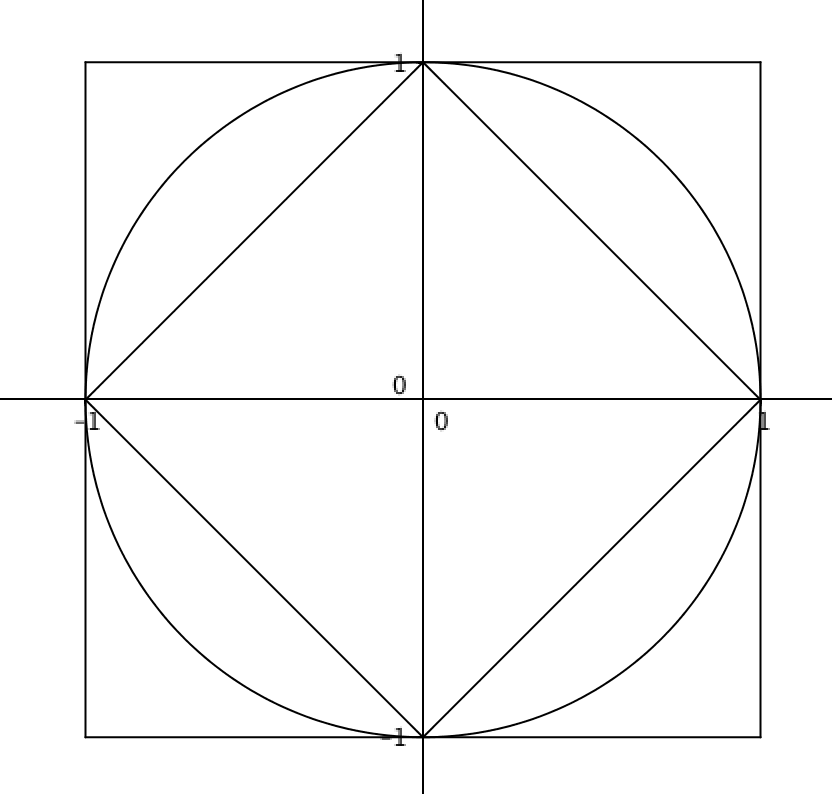
\includegraphics[scale=0.4]{Boulesunites}
%\end{center}
\end{Exemple}

\subsection{Suites d'éléments d'un espace vectoriel}

\begin{Definition}{} Soit $E$ un espace vectoriel. 

On appelle \emph{suite} d'éléments de $E$ toute application $u : \mathbb{N} \rightarrow E$. Pour tout $n \in \mathbb{N}$, on note $u_n$ au lieu de $u(n)$ : ce vecteur est le terme de rang $n$ de cette suite. On note la suite $(u_n)_{ n \geq 0}$ ou $(u_n)$.
\end{Definition}

\begin{Remarques}{}
\begin{itemize} 
\item Une suite peut être définie uniquement à partir d'un rang $n_0 \geq 1$.
\item On peut définir des suites extraites, comme dans le cas où $E = \mathbb{K}$.
\end{itemize}
\end{Remarques}{}

\medskip

\begin{Exemple} Soient $p \in \mathbb{N}^{*}$ et $A \in \mathcal{M}_p(\mathbb{K})$. On définit une suite $(u_n)_{n \geq 0}$ d'éléments de $\mathcal{M}_p(\mathbb{K})$ en posant pour tout $n \geq 0$, $u_n = A^n$. 
\end{Exemple}

\subsection{Normes équivalentes}

\begin{Definition}{} Deux normes sur $E$, $N_1$ et $N_2$, sont équivalentes si :

\vspace{1cm}
\end{Definition}

\begin{Exemple} Montrons que les normes $1$, $2$ et infini sont \emph{équivalentes} sur $\mathbb{R}^n$ :

\vspace{7cm}
\end{Exemple}

\begin{Theoreme}{Admis} Dans un espace vectoriel de dimension finie, les normes sont équivalentes.
\end{Theoreme}

\subsection{Ensembles, suites et fonctions bornés}

Dorénavant, l'espace vectoriel $E$ sera de \emph{dimension finie}.

\begin{Definition}{}
Soit $(E, \Vert \cdot \Vert)$ un espace vectoriel normé.

\begin{enumerate}
\item Si $A$ est une partie de $E$, on dit que $A$ est \emph{bornée} si il existe un réel $M \geq 0$ tel que pour tout $a \in A$, $\Vert a \Vert \leq M$, ce qui équivalent à $A \subset B_f(0_E,M)$.
\item Si $(u_n)_{n \geq 0}$ est une suite de $E$, on dit que $(u_n)_{n \geq 0}$ est \emph{bornée} si $\lbrace u_n \, \vert \, n \geq 0\rbrace$ est bornée.

% ce qui équivalent à l'existence d'un réel $M \geq 0$ tel que pour tout $n \geq 0$, $\Vert u_n \Vert \leq M$.
\item Si $X$ est un ensemble non vide et $f : X \rightarrow E$ une application, on dit que $f$ est \emph{bornée} si $\lbrace f(x) \, \vert \, x \in X \rbrace$ est bornée.
% ce qui équivalent à l'existence d'un réel $M \geq 0$ tel que pour tout $x \in X$, $\Vert f(x) \Vert \leq M$.
\end{enumerate}
\end{Definition}

\medskip

Ainsi, $(u_n)_{n \geq 0}$ est bornée si et seulement si :

\vspace{1cm}

et $f : X \rightarrow E$ est bornée si et seulement si :

\vspace{1.3cm}

\begin{Theoreme}{} Les définitions précédentes ne dépendent pas de la norme utilisée car $E$ est de dimension finie.
\end{Theoreme}

\begin{Demonstration}{} Conséquence directe du fait que les normes sont équivalentes sur $E$.
\end{Demonstration}

\medskip

\begin{Exemples}
\begin{enumerate}
\item Une boule ouverte d'un espace vectoriel normé $(E, \Vert \cdot \Vert)$ est bornée : pour $a \in E$ et $r \in \mathbb{R}_+$, on a pour tout $x \in B(a,r)$, par l'inégalité triangulaire,
%$$ \Vert x \Vert = \Vert x-a + a \Vert \leq \Vert x - a \Vert + \Vert a \Vert \leq r+ \Vert a \Vert$$
%En posant $M = r+ \Vert a \Vert$, la définition est vérifiée.

\vspace{2cm}
On montre de même qu'une boule fermée ou qu'une sphère est bornée.
\item Soit $A = \lbrace (x,y) \in (\mathbb{R}^+)^2 \, \vert \, x+2y \leq 5 \rbrace$. Montrons que $A$ est bornée dans $\mathbb{R}^2$.

\vspace{4cm}
%\item Considérons $\mathcal{B}(\mathbb{R}_+, \mathbb{R})$ muni de la norme infini. On pose pour tout $n \geq 0$ et tout $x \in \mathbb{R}_+$,
%$$ f_n(x) = e^{-nx}$$
%On crée ainsi une suite $(f_n)_{n \geq 0}$ d'éléments de $\mathcal{B}(\mathbb{R}_+, \mathbb{R})$ et il est clair que pour tout $n \geq 0$, $\Vert f_n \Vert_{\infty} = 1$ donc cette suite est bornée.
%\item \textbf{METTRE EXEMPLE DANS R2 ou R3}
\item Posons :
$$ \begin{array}{ccccl}
f & : & ]0,1]^2 & \rightarrow & \mathbb{R}^2 \\
& & (x,y)   & \mapsto & (\ln(xy), \cos(x)+ \sin(y)) \\
\end{array}$$
Montrons que $f$ n'est pas bornée : 

\vspace{4cm}
%pour tout $x \in ]0,1[$, $f(x,1) = (\ln(x),\cos(x) + \sin(1))$ donc :
%$$ \Vert f(x,1) \Vert_1 = \vert \ln(x) \vert + \vert \cos(x) + \sin(1) \vert \geq -\ln(x) -1  + \sin(1)$$
%Or $\lim_{x \rightarrow 0}  -\ln(x) -1  + \sin(1) = + \infty$ donc la définition de $f$ bornée ne peut être vérifiée pour aucun réel positif $M$.
\end{itemize}
\end{Exemples}

\begin{ApplicationDirecte} Montrer que $A = \lbrace (x,y)\in\R^2 \, \vert \, x^2+y^4=1 \rbrace$ est bornée dans $\mathbb{R}^2$.
\end{ApplicationDirecte}

\subsection{Parties convexes}

\begin{Definition}{} Soit $C$ une partie d'un espace vectoriel $E$. On dit que $C$ est \emph{convexe} si :

\vspace{1cm}

%pour tout $(x,y) \in C^2$ et pour tout $\lambda \in [0,1]$, $\lambda x + (1- \lambda)y \in C$. 
\end{Definition}

\begin{Remarques}{}
\begin{itemize} 
\item $C$ est convexe si et seulement si il contient tout segment dont il contient les extrémités.
\item La notion d'ensemble convexe ne fait pas intervenir de norme.
\end{itemize}
\end{Remarques}{}

\begin{center}
\emph{Une partie non convexe et une partie convexe de $\mathbb{R}^2$.}
\end{center}

\begin{center}
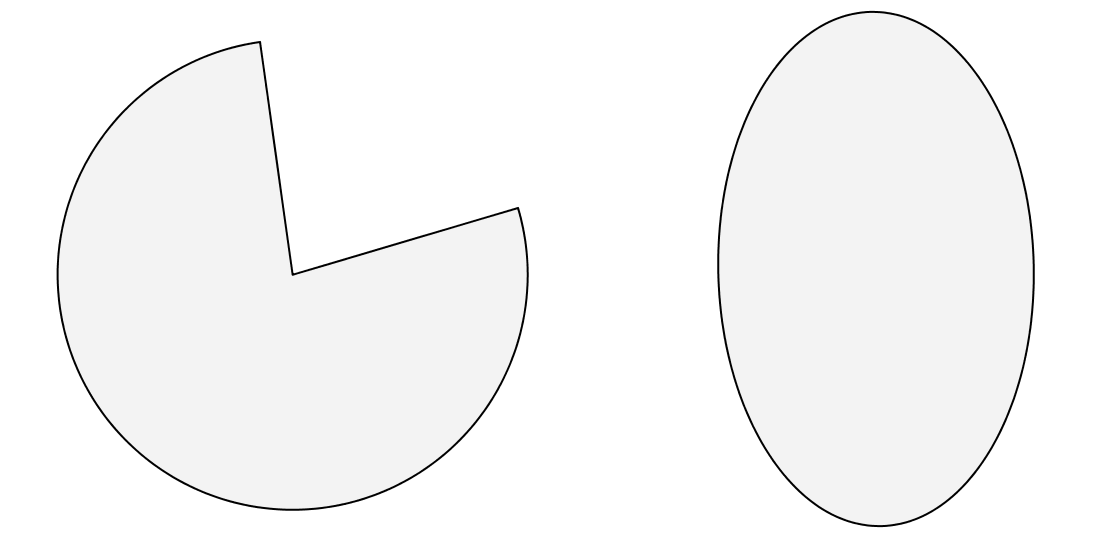
\includegraphics[scale=0.5]{Convexes}
\end{center}

\textbf{Exemple important : les boules unités fermées ou ouvertes sont convexes.}


\vspace{6cm}
%Fixons $a \in E$ et $r \in \mathbb{R}_+$. Soient $(x,y) \in B(a,r)^2$ et $\lambda \in [0,1]$. On a :
%
%\begin{align*}
%\Vert \lambda x+ (1-\lambda y) - a \Vert  & = \Vert \lambda x+ (1-\lambda) y - (\lambda + (1 - \lambda))a \Vert \\
%& = \Vert \lambda (x-a) + (1- \lambda) (y-a) \Vert \\
%& \leq  \Vert \lambda (x-a) \Vert + \Vert (1- \lambda) (y-a) \Vert \qquad \hbox{(inégalité triangulaire)} \\
%& =  \lambda \Vert x-a \Vert + (1-\lambda) \Vert y-a \Vert  \qquad \hbox{(car } \lambda \geq 0 \hbox{ et } 1-\lambda \geq 0) \\
%& < \lambda r + (1-\lambda r) \qquad \hbox{(car } x \in B(a,r) \hbox{ et } y \in B(a,r)) \\
%& = 1 \\
%\end{align*}
%Ainsi $\lambda x+ (1-\lambda y) \in B(a,r)$. On a donc bien montré que $B(a,r)$ était convexe (même preuve pour $B_f(a,r)$).

\begin{ApplicationDirecte} Pacman est-il convexe ?
\end{ApplicationDirecte} 

\section{Convergence de suites}
\subsection{Définition}
\begin{Definition}{} Soit $(u_n)_{n \geq 0}$ une suite d'éléments d'un espace vectoriel normé $(E, \Vert \cdot \Vert)$.

\begin{itemize}
\item Soit $\ell \in E$. On dit que $(u_n)_{ n\geq 0}$ \emph{converge} vers $\ell$ (ou que $u_n$ tend vers $\ell$ quand $n$ tend vers $+ \infty$) si :

\vspace{1cm}

%$$ \forall \varepsilon >0, \, \exists N \in \mathbb{N} \, \vert \, \forall n  \geq N, \, \Vert u_n - \ell \Vert  \leq \varepsilon$$
\item La suite $(u_n)$ est dite \emph{convergente} si il existe un vecteur $\ell \in E$, appelé \emph{limite}, tel que $(u_n)_{n \geq 0}$ converge vers $\ell$.
\item Si une suite ne converge pas, on dit qu'elle \emph{diverge}.
\end{itemize}
\end{Definition}

\begin{Theoreme}{} Si une suite d'éléments d'un espace vectoriel normé converge, il y a \emph{unicité} de la limite. On note celle-ci $\lim_{n \rightarrow + \infty} u_n$.
\end{Theoreme}

\begin{Remarque}{} $(u_n)_{n \geq 0}$ converge vers $\ell$ si et seulement si $\Vert u_n - \ell \Vert$ tend vers $0$ quand $n \rightarrow + \infty$.  Cette remarque à deux intérêts : se ramener à une suite de réels positifs et montrer que celle-ci converge vers $0$ (ce qui est plus simple que de montrer qu'une suite tend vers un vecteur quelconque) même si il faut avoir de l'intuition pour déterminer la limite.
\end{Remarque}

\begin{Theoreme}{} La notion de convergence de suite ne dépend pas de la norme choisie si l'on travaille sur un espace vectoriel de \emph{dimension finie}.
\end{Theoreme}

\begin{Demonstration}{} Conséquence directe du fait que les normes sont équivalentes sur un espace de dimension finie.
\end{Demonstration}

\begin{Exemple} Posons pour tout $n \geq 1$, $u_n = \left( \dfrac{1}{n}, \dfrac{1}{n^2} \right)$. Alors $(u_n)_{n \geq 1}$ est une suite d'éléments de $\mathbb{R}^2$. Étudions sa convergence.

%\medskip
%
%$\rhd$ Considérons la norme 1 : il semble intuitif de dire que cette suite converge vers $(0,0)$. Pour tout $n \geq 1$,
%$$ \Vert u_n - (0,0) \Vert_{1} = \phantom{\left\Vert \left(  \dfrac{1}{n}, \dfrac{1}{n^2} \right) \right\Vert_{1} = \dfrac{1}{n} + \dfrac{1}{n^2}  \underset{n \rightarrow + \infty}{\longrightarrow} 0}$$
%Ainsi, la suite $(u_n)_{n \geq 1}$ converge vers $(0,0)$ dans $(\mathbb{R}^2, \Vert \cdot \Vert_{1})$.
%
%\medskip
%
%$\rhd$ Considérons la norme infini : il semble intuitif de dire que cette suite converge vers $(0,0)$. Pour tout $n \geq 1$,
%$$ \Vert u_n - (0,0) \Vert_{ \infty} = \phantom{\left\Vert \left(  \dfrac{1}{n}, \dfrac{1}{n^2} \right) \right\Vert_{\infty} = \max\left( \dfrac{1}{n}, \dfrac{1}{n^2} \right) = \dfrac{1}{n}  \underset{n \rightarrow + \infty}{\longrightarrow} 0}$$
%Ainsi, la suite $(u_n)_{n \geq 1}$ converge vers $(0,0)$ dans $(\mathbb{R}^2, \Vert \cdot \Vert_{\infty})$.

\vspace{6cm}
\end{Exemple}

%La définition de convergence dépend à priori de la norme employée sur l'espace. Le théorème suivant (que nous admettons) est crucial pour la suite.
%
%\begin{Theoreme}{} La notion de convergence de suite ne dépend pas de la norme choisie si l'on travaille sur un espace vectoriel de \emph{dimension finie}.
%\end{Theoreme}

\begin{Exemple} Pour étudier la convergence d'une suite d'éléments de $\mathbb{K}^n$ avec $n \in \mathbb{N}^*$, on peut utiliser la norme que l'on souhaite (par exemple la norme $1$, la norme $2$ ou la norme infini). L'idée de la preuve dans ce cadre précis est qu'il est facile de comparer les boules pour ces trois normes.
\end{Exemple}

\begin{Proposition}{} Soit $(u_n)_{n \geq 0}$ une suite d'éléments d'un espace vectoriel normé $(E, \Vert \cdot \Vert)$.

\begin{itemize}
\item Si $(u_n)_{n \geq 0}$ converge, elle est bornée.
\item Si $(u_n)_{n \geq 0}$ converge, ses suites extraites convergent aussi et vers la même limite.
\end{itemize}
\end{Proposition}

\begin{Proposition}{} L'ensemble des suites convergentes d'éléments de $E$ est un sous-espace vectoriel de l'ensemble des suites de $E$. Ainsi, si $(u_n)_{n \geq 0}$ et $(v_n)_{n \geq 0}$ sont deux suites convergentes de $E$, convergeant vers $\ell$ et $\ell'$ et si $(\lambda, \mu) \in \mathbb{K}^2$ alors $(\lambda u_n + \mu v_n)_{n \geq 0}$ est convergente et converge vers $\lambda \ell + \mu \ell'$.
\end{Proposition}


\subsection{Lien entre convergence et suites coordonnées}

Fixons dans cette section un espace vectoriel $E$ de dimension finie $p \in \mathbb{N}^*$ et $\mathcal{B} = (e_1, \ldots, e_p)$ une base de $E$. Tout vecteur $x$ a des coordonnées $(x_1, \ldots, x_p)$ dans cette base $\mathcal{B}$. 

Soit $(u_n)_{n \geq 0}$ une suite d'éléments de $E$. Pour tout $n \geq 0$, $u_n$ a des coordonnées $((u_{n,1}, \ldots, u_{n,p}))$ dans $\mathcal{B}$ ce qui est équivalent à dire que :
$$ u_n = u_{n,1} e_1 + \cdots + u_{n,p} e_p $$

\begin{Exemple} Si $(e_1,e_2)$ est la base canonique de $\mathbb{R}^2$, on a pour tout $n \geq 0$,
$$ (\sin(n),n^2) = \sin(n) e_1 + n^2e_2$$
\end{Exemple}

\begin{Theoreme}{} En gardant les notations précédentes, les assertions suivantes sont équivalentes :
\begin{itemize}
\item La suite $(u_n)_{n \geq 0}$ converge.
\item Pour tout $i \in \Interv{1}{p}$, la suite $(u_{n,i})_{n \geq 0}$ converge.
\end{itemize}
Quand celles-ci sont vraies, on a :
$$ \lim_{n \rightarrow + \infty} u_n = \sum_{i=1}^p \left(\lim_{n \rightarrow + \infty} u_{n,i} \right) e_i $$
\end{Theoreme}

\begin{Demonstration}{} Voir TD.
\end{Demonstration}

%\begin{Demonstration}{} Nous commençons par montrer un résultat préliminaire puis nous montrons le résultat pas double implications.
%
%\medskip
%
%$\rhd$ Tout vecteur $x$ de $E$ a des coordonnées $(x_1, \ldots, x_p)$ dans cette base $\mathcal{B}$. On pose alors :
%$$ \Vert x \Vert_1 = \sum_{i=1}^p \vert x_i \vert \quad \hbox{ et } \Vert x \Vert_{\infty} = \max_{1 \leq i \leq p} \vert x_i \vert $$
%On vérifie que cela définit deux normes sur $E$ (preuves équivalentes à celles effectuées sur $\mathbb{K}^n$).
%
%\medskip
%
%$\rhd$ Supposons que la suite $(u_n)_{n \geq 0}$ converge vers un vecteur $\ell = (\ell_1, \ldots, \ell_p)$ de $E$.
%
%
%%En utilisant la norme infini (légitime car $E$ est de dimension finie) on a alors :
%%$$ \lim_{n \rightarrow + \infty} \Vert u_n - \ell \Vert_{\infty} = 0$$
%%ou encore :
%%$$ \lim_{n \rightarrow + \infty} \left( \max_{1 \leq i \leq n} \vert u_{n,i}- \ell_i \vert \right)$$
%%Or, pour tout $i \in \Interv{1}{p}$ et tout $n \geq 0$,
%%$$ 0 \leq \vert u_{n,i}- \ell_i \vert \leq \max_{1 \leq i \leq n} \vert u_{n,i}- \ell_i \vert $$
%%Par théorème d'encadrement, la suite de terme général $ \vert u_{n,i}- \ell_i \vert $ converge donc vers $0$ et ainsi $(u_{n,i})_{n \geq 0}$ converge vers $\ell_i$.
%
%\vspace{7cm}
%
%\medskip
%
%$\rhd$ Supposons que pour tout $i \in \Interv{1}{p}$, la suite $(u_{n,i})_{n \geq 0}$ converge vers un scalaire $\ell_i$.
%
%% Considérons la norme $1$ (légitime car $E$ est de dimension finie). On a pour tout $i \in \Interv{1}{p}$,
%%$$ \lim_{n \rightarrow + \infty} \vert u_{n,i} - \ell_i \vert = 0$$
%%Ainsi, par somme de suites convergentes :
%%$$ \Vert u_n - \ell \Vert_{1} = \sum_{i=1}^p \vert u_{n,i} - \ell_i \vert  \underset{n \rightarrow + \infty}{\longrightarrow} 0$$
%%Ainsi $(u_n)_{n \geq 0}$ converge vers $\ell = (\ell_1, \ldots, \ell_p)$.
%
%\vspace{7cm}
%\end{Demonstration}

\begin{ApplicationDirecte} Calculer $\lim_{n \rightarrow + \infty} \begin{pmatrix}
\frac{1}{n} & \cos \left( \frac{1}{n} \right) \\
1 & arctan(n) \\
\end{pmatrix}$ (des normes sur des espaces de matrices sont données en TD).
\end{ApplicationDirecte}

\section{Topologie d'un espace vectoriel de dimension finie}

\subsection{Ouvert}

\begin{Theoreme}{} On admet que toutes les définitions et résultats de cette section ne dépendent pas de la norme car $E$ est de dimension finie (ce qui implique que les normes sont équivalentes sur $E$).
\end{Theoreme}

\begin{Definition}{} Soient $(E, \Vert \cdot \Vert)$ un espace vectoriel normé, $A$ une partie de $E$ et $a \in A$. On dit que $a$ est un \emph{point intérieur} de $A$ si :

\vspace{1cm}
% il existe un réel $r>0$ tel que $B(a,r) \subset A$.
\end{Definition}

\begin{Remarque}{} Un vecteur $a$ est un point intérieur de $A$ si et seulement si :
$$ \exists r>0, \, \forall x \in E, \, \Vert x-a \Vert < r \Rightarrow x \in A$$
\end{Remarque}

\begin{center}
\emph{Un exemple de point intérieur}

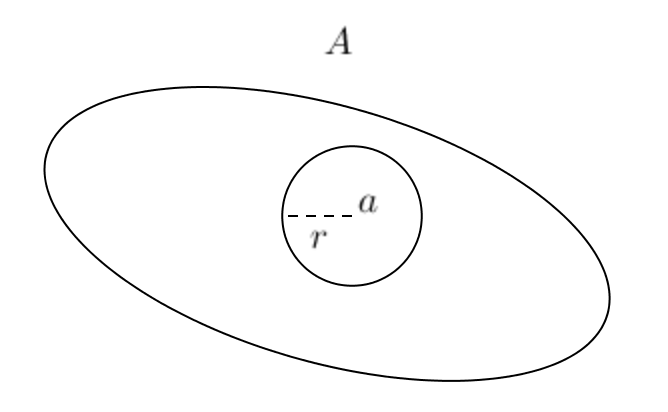
\includegraphics[scale=0.5]{Ouvert}
\end{center}

\begin{Exemple} Soit $(u_n)_{n \geq 0}$ une suite d'éléments d'un espace vectoriel normé $(E, \Vert \cdot \Vert)$ convergeant vers un point intérieur $a$ d'une partie $A$ de $E$. Montrons qu'à partir d'un certain rang, tous les termes de la suite sont dans $A$.


\vspace{3cm}
%\medskip
%
%Le point $a$ étant intérieur, il existe un réel $r>0$ tel que pour tout $x \in E$, si $\Vert x- a \Vert<r$ alors $x \in A$. La suite $(u_n)_{n \geq 0}$ converge vers $a$ donc par définition de la convergence (en prenant $\varepsilon=r>0$), il existe un rang $N \in \mathbb{N}$ tel que pour tout entier $n \geq N$, $\Vert u_n -a \Vert <r$ et ainsi pour tout $n \geq N$, $u_n \in A$.
\end{Exemple}

\begin{ApplicationDirecte} Représenter graphiquement l'ensemble suivant de $\mathbb{R}^2$ :
$$ A= \lbrace (x,y) \in \mathbb{R}^2 \, \vert \,  y \geq x^2 \hbox{ et } y \leq 2 \rbrace$$
Justifier graphiquement que $(0,1)$ est un point intérieur de $A$ mais que $(1,1)$ n'en est pas un.
\end{ApplicationDirecte}

\begin{Definition}{} Soient $(E, \Vert \cdot \Vert)$ un espace vectoriel normé et $A$ une partie de $E$. On appelle \emph{intérieur} de $A$, et on note $\mathring{A}$, l'ensemble des points intérieurs de $A$.
\end{Definition}

\begin{Remarque}{} Les points intérieurs de $A$ sont en particulier des points de $A$ donc $\mathring{A} \subset A$.
\end{Remarque}

\begin{Exemple} Si $A=[0,1]$, $\mathring{A} = ]0,1[$.
\end{Exemple}

\begin{Definition}{}
Soient $(E, \Vert \cdot \Vert)$ un espace vectoriel normé et $A$ une partie de $E$. On dit que $A$ est un \emph{ouvert} de $E$ si $\mathring{A}=A$, c'est-à-dire si tous les éléments de $A$ sont des points intérieurs de $A$. Autrement dit si :
$$ \phantom{\forall a \in A, \, \exists r>0 \, \vert \, B(a,r) \subset A}$$
\end{Definition}
%
%\begin{Proposition}{} On admet que si $E$ est de dimension finie, la notion de point intérieur et la notion d'ouverts ne dépend pas de la norme choisie. On ne précisera donc pas la norme.
%\end{Proposition}

\begin{Exemples}
\begin{enumerate}
\item $E$ et $\varnothing$ sont des ouverts de $E$.
\item Les intervalles ouverts de $\mathbb{R}$ sont des ouverts de $\mathbb{R}$.
\item On admet que le produit cartésien d'ouverts est un ouvert. Par exemple $]-1,1[ \times \mathbb{R}_{+}^*$ est un ouvert de $\mathbb{R}^2$.
\end{itemize}
\end{Exemples}

\medskip

\textbf{Exemple important : les boules ouvertes sont des ouverts.}

Soient $(E, \Vert \cdot \Vert)$ un espace vectoriel normé, $a \in E$, $r \in \mathbb{R}_+^*$. Soit $b \in B(a,r)$. Représentons cela sur un dessin :

\begin{center}
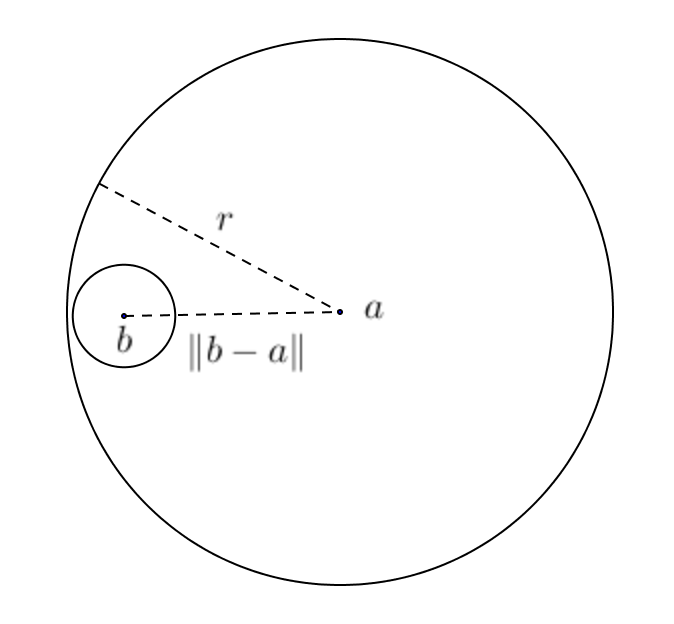
\includegraphics[scale=0.4]{BouleOuv}
\end{center}

\vspace{4cm}

%
%Posons $\varepsilon = r - \Vert b-a \Vert$. Alors $\varepsilon>0$ car $b \in B(a,r)$ et pour tout $x \in B(b, \varepsilon)$, on a :
%$$ \Vert  x - a \Vert  = \Vert  x - b + b- a \Vert \leq \Vert  x - b \Vert + \Vert  b - a \Vert <\varepsilon + \Vert  b - a \Vert =  r$$
%et donc $x \in  B(a,r)$. On a ainsi $B(b, \varepsilon) \subset B(a,r)$ et $B(a,r)$ est donc un ouvert.

\subsection{Fermé}

\begin{Theoreme}{} On admet que toutes les définitions et résultats de cette section ne dépendent pas de la norme car $E$ est de dimension finie (donc les normes sont équivalentes sur cet espace).
\end{Theoreme}

%\begin{Theoreme}{} On admet que toutes les définitions et résultats de cette section ne dépendent de la norme car $E$ est de dimension finie.
%\end{Theoreme}

\begin{Definition}{} 
Soient $(E, \Vert \cdot \Vert)$ un espace vectoriel normé, $A$ une partie de $E$ et $a \in E$. On dit que $a$ est un \emph{point adhérent} de $A$ si :
\vspace{1cm}
%
%pour tout réel $r>0$, $B(a,r) \cap A \neq \varnothing$.
\end{Definition}

\begin{Remarques}{}
\begin{itemize} 
\item Tout élément de $A$ est adhérent à $A$ (car pour tout $a \in A$ et $r>0$, $B(a,r) \cap A$ contient $a$).
\item $-1$ est adhérent à $]-1,1[$.
\end{itemize}
\end{Remarques}{}

\begin{Proposition}{} Soit $(E, \Vert \cdot \Vert)$ un espace vectoriel normé, $A$ une partie de $E$ et $a \in E$. Les assertions suivantes sont équivalentes :

\begin{enumerate}
\item Le point $a$ est adhérent à $A$.
\item Il existe une suite d'éléments de $A$ qui converge vers $a$.
\end{enumerate}
\end{Proposition}

\begin{Demonstration}{} On procède par double implications.
%
%$\rhd$ Supposons que le point $a$ est adhérent à $A$. Pour tout entier naturel $n \geq 1$, on a $B(a, \frac{1}{n}) \cap A \neq \varnothing$ et ainsi il existe $x_n \in B(a,\frac{1}{n}) \cap A$. On a donc pour tout $n \geq 1$,
%$$ \Vert x_n - a \Vert \leq \frac{1}{n}$$
%Par Théorème d'encadrement, on montre que $x_n \underset{n \rightarrow + \infty}{\rightarrow} a$ et cette suite est bien une suite d'éléments de $A$.
%
%\medskip
%
%$\rhd$ Supposons l'existence d'une suite $(x_n)_{n \geq 0}$ d'éléments de $A$ qui converge vers $a$. Fixons $r > 0$. Par définition de la convergence, pour $n$ assez grand, on a :
%$$ \Vert x_n - a \Vert < r $$
%et ainsi $x_n \in B(a,r) \cap A$ et en particulier $B(a,r) \cap A \neq \varnothing$.

\vspace{10cm}
\end{Demonstration}

%\newpage
%$\phantom{}$

%\vspace{7cm}

\begin{Exemple} Montrons que la matrice $\begin{pmatrix}
0 & 1 \\
0 & 0 \\
\end{pmatrix}$ est adhérente à l'ensemble des matrices inversibles de $\mathcal{M}_2(\mathbb{R})$ :

\vspace{3cm}
%
% (carrées d'ordre $2$). En effet, on a :
%$$A_n = \begin{pmatrix}
%\frac{1}{n} & 1 \\
%0 & \frac{1}{n} \\
%\end{pmatrix} \underset{n \rightarrow + \infty}{\rightarrow}  \begin{pmatrix}
%0 & 1 \\
%0 & 0 \\
%\end{pmatrix}$$
%et chacune des matrices $A_n$ (pour $n \geq 1$) est inversible car triangulaire supérieure avec des coefficients diagonaux non nuls.
\end{Exemple}

\begin{Definition}{} Soient $(E, \Vert \cdot \Vert)$ un espace vectoriel normé et $A$ une partie de $E$. On appelle \emph{adhérence} de $A$ l'ensemble, noté $\overline{A}$, des points adhérents de $A$.
\end{Definition}

\begin{Remarques}{}
\begin{itemize}
\item On a toujours $A \subset \overline{A}$.
\item L'adhérence de $[-1,1[$ est $[-1,1]$.
\end{itemize}
\end{Remarques}{}

\begin{Definition}{} Soient $(E, \Vert \cdot \Vert)$ un espace vectoriel normé et $A$ une partie de $E$. On dit que $A$ est \emph{fermé} si tous les points adhérents de $A$ appartiennent à $A$. Autrement dit, $A$ est fermé si $\overline{A}=A$.
\end{Definition}

\begin{Exemples}
\begin{enumerate}
\item L'ensemble $[-1,1[$ n'est pas un fermé.
\item Pour tout $A \subset E$, $\overline{A}$ est un fermé.
\end{itemize}
\end{Exemples}

\begin{Proposition}{} Soient $(E, \Vert \cdot \Vert)$ un espace vectoriel normé et $A$ une partie de $E$. Les propositions suivantes sont équivalentes :
\begin{enumerate}
\item $A$ est une partie fermée.
\item Pour toute suite convergente $(x_n)_{n \geq 0}$ d'éléments de $A$, on a $\lim_{n \rightarrow + \infty} x_n \in A$.
\end{enumerate}
\end{Proposition}


\begin{Proposition}{} Soit $(E, \Vert \cdot \Vert)$ un espace vectoriel normé, $A$ une partie de $E$. Alors $A$ est fermée si et seulement si son complémentaire est une partie ouverte.
\end{Proposition}

\begin{Demonstration}{} Raisonnons par double implications.
%
%$\rhd$ Supposons que $A$ est fermé et montrons que $^cA$ est ouvert. Soit $a \in ^cA$. Montrons l'existence d'un réel strictement positif $r$ tel que $B(a,r) \subset ^cA$. Si ce n'est pas le cas, pour tout $r>0$, il existe $x \in B(a,r)$ tel que $x \notin ^cA$. Ainsi, pour tout $r>0$, il existe $x \in B(a,r)$ tel que $x \in A$. Ainsi $a$ est adhérent à $A$ qui est fermé donc $a \in A$ ce qui est absurde.
%
%\medskip 
%
%$\rhd$ Supposons que $^cA$ soit un ouvert. Montrons que $A$ est fermé. Soit $a \in \overline{A}$ : si $a \notin A$ alors $a \in ^cA$ qui est ouvert donc il existe un réel strictement positif $r$ tel que $B(a,r) \subset ^cA$. Or $a$ un est un point adhérent à $A$ donc il existe un élément $x \in A$ tel que $x B(a,r)$ ce qui est absurde.

\vspace{10cm}
\end{Demonstration}

%\newpage
%
%\phantom{test}
%
%\vspace{5cm}

\begin{Corollaire}{} Les boules fermées et les sphères sont fermées.
\end{Corollaire}

\begin{Demonstration}{}

\vspace{8cm}

\end{Demonstration}



\subsection{Frontière d'une partie}

\begin{Definition}{} Soit $A$ une partie de $E$. On appelle \emph{frontière} de $A$, et on note $\textrm{Fr}(A)$, l'ensemble de ses points adhérents qui ne sont pas intérieurs. Autrement dit, $\textrm{Fr}(A) = \overline{A} \setminus \mathring{A}$.
\end{Definition} 

\begin{Exemple} La frontière de $[0,1]$ est $\lbrace 0,1 \rbrace$ et la frontière d'une boule fermée est la sphère associée.
\end{Exemple}

\section{Fonctions entre espaces vectoriels normés}

Dans la suite, on considère $(E, \Vert \cdot \Vert_E)$ et $(F, \Vert \cdot \Vert_F)$ deux espaces vectoriels normés de dimension finie et une fonction $f : A \subset E \rightarrow B \subset F$.

\begin{Theoreme}{} Les résultats de toute cette section ne dépendent pas de la norme choisie car les espaces sont de dimensions finies (donc les normes sont équivalentes sur ceux-ci).
\end{Theoreme}


\begin{TheoremeDefinition}{} Soient $a \in \overline{A}$ et $b \in F$.

\begin{itemize}
\item On dit que $f$ a un pour limite $b$ en $a$ (ou que $f(x)$ tend vers $b$ quand $x$ tend vers $a$) si :
$$ \forall \varepsilon >0, \, \exists \eta > 0, \, \forall x \in A, \, \Vert x- a \Vert_E \leq \eta \Rightarrow \Vert f(x) - b \Vert_F \leq \varepsilon$$
\item Si $f$ admet une limite $b$ en $a$, celle-ci est unique. On l'appelle \emph{limite} de $f$ en $a$ et on note $\lim_{x \rightarrow a} f(x) = b$ ou encore $f(x) \underset{x \rightarrow a}{\rightarrow} b$.
\end{itemize}
\end{TheoremeDefinition}

\begin{Remarque}{} L'intérêt de choisir $a \in \overline{A}$ est d'être sur de l'existence d'éléments de $A$ \og proche \fg de $a$.
\end{Remarque}

\begin{Definition}{} Soient $m \in \mathbb{R}$, $f$ une fonction définie sur $]m, + \infty[$ à valeurs dans $F$ et $b \in F$.

On dit que $f$ a pour limite $b$ en $+ \infty$ si :
$$ \forall \varepsilon>0, \exists M \in \mathbb{R}, \, \forall x \in ]m, + \infty[, \, x \geq M \Rightarrow \Vert f(x)- b \Vert_F \leq \varepsilon$$
 Si $f$ admet une limite $b$ en $+ \infty$, celle-ci est unique. On l'appelle \emph{limite} de $f$ en $+ \infty$ et on note \newline $\lim_{x \rightarrow + \infty} f(x) = b$ ou encore $f(x) \underset{x \rightarrow + \infty}{\rightarrow} b$.
\end{Definition}

\begin{Remarque}{} On définit de même la limite en $- \infty$ d'une fonction si celle-ci est définie sur un intervalle de la forme $]- \infty, m[$ où $m \in \mathbb{R}$.
\end{Remarque}
%
%\begin{Definition}{} Soient $m \in \mathbb{R}$, $f$ une fonction définie sur $]- \infty, m[$ à valeurs dans $F$ et $b \in F$.
%
%On dit que $f$ a pour limite $b$ en $- \infty$ si :
%$$ \forall \varepsilon>0, \exists M \in \mathbb{R}, \, \forall x \in ]- \infty, m[, \, x \leq M \rightarrow \Vert f(x)- b \Vert_F \leq \varepsilon$$
% Si $f$ admet une limite $b$ en $- \infty$, celle-ci est unique. On l'appelle limite de $f$ en $- \infty$ et on note \newline $\lim_{x \rightarrow - \infty} f(x) = b$ ou encore $f(x) \underset{x \rightarrow - \infty}{\rightarrow} b$.
%\end{Definition}

\begin{Definition}{} Soient $f$ une fonction définie sur $A$ et à valeurs réelles et $a \in \overline{A}$. On dit que $f$ admet $+ \infty$ en $a$ si :
$$ \forall M \in \mathbb{R}, \, \exists r > 0, \, \forall x \in A, \, x \in B(a,r) \Rightarrow f(x) \geq M$$
%\item On dit que $f$ admet $- \infty$ en $a$ si :
%$$ \forall M \in \mathbb{R}, \, \exists r > 0, \, \forall x \in A, \, x \in B(a,r) \Rightarrow f(x) \leq M$$
%\end{itemize}
Il y a aussi dans ce cas l'unicité de la limite.
\end{Definition}

\begin{Remarque}{} On définit de même le fait que $f$ admette $- \infty$ comme limite en $a$.
\end{Remarque}

\subsection{Continuité}

\begin{TheoremeDefinition}{} On dit que $f$ est \emph{continue} en $a$ si la limite de $f$ en $a$ existe. Dans ce cas, on a nécessairement :
$$ \lim_{x \rightarrow a} f(x) = f(a) $$
\end{TheoremeDefinition}

\begin{Definition}{} On dit que $f$ est continue sur $A$ si $f$ est continue en tout point de $A$.
\end{Definition}

\subsection{Caractérisation séquentielle}

\begin{Proposition}{} Soient $a \in \overline{A}$ et $\ell \in F$. Les assertions suivantes sont équivalentes :

\begin{enumerate}
\item La limite de $f$ en $a$ existe et vaut $\ell$.
\item Pour toute suite $(a_n)_{n \geq 0}$ d'éléments de $A$ convergente vers $a$, $(f(a_n))_{n \geq 0}$ converge vers $\ell$.
\end{enumerate}
\end{Proposition}

\begin{Demonstration}{} Équivalente à celle donnée en première année dans le cas des fonctions de la variable réelle et à valeurs réelles.
\end{Demonstration}

%$\rhd$ Supposons que la limite de $f$ en $a$ existe et soit égale à $\ell$ et fixons une suite $(a_n)_{n \geq 0}$ d'éléments de $A$ convergente vers $a$. 
%
%\newpage
%$\phantom{test}$
%%Soit $\varepsilon>0$. On cherche l'existence d'un entier $N$ tel que pour entier $n \geq N$,
%%$$ \Vert f(a_n) - \ell \Vert_F \leq \varepsilon$$
%%La limite de $f$ en $a$ étant égale à $\ell$, il existe un réel $r>0$ tel que pour tout $x \in A$,
%%$$ \Vert x - a \Vert_E \leq r \Rightarrow \Vert f(x) - \ell \Vert_F \leq \varepsilon$$
%%Or la suite $(a_n)_{n \geq 0}$ converge vers $a$ donc il existe un entier $N \geq 0$ tel que pour tout entier $n \geq N$,
%%$$ \Vert a_n - a \Vert_E \leq r$$
%%Finalement, pour tout $n \geq N$, $\Vert a_n - a \Vert_E \leq r$ et ainsi $\Vert f(a_n) - \ell \Vert_F \leq \varepsilon$.
%%
%%On a ainsi montré que $(f(a_n))_{n \geq 0}$ convergeait vers $\ell$.
%
%
%\vspace{7cm}
%
%$\rhd$ Supposons que pour toute suite $(a_n)_{n \geq 0}$ d'éléments de $A$ convergente vers $a$, $(f(a_n))_{n \geq 0}$ converge vers $\ell$. Supposons par l'absurde que $f$ n'admette pas $\ell$ pour limite en $a$.
%%
%% On a alors :
%%$$ \exists \varepsilon > 0, \, \forall r > 0, \, \exists x \in A, \, \Vert x-a \Vert_E < r \hbox{ et } \Vert f(x) - \ell \Vert_F > \varepsilon$$
%%Ainsi, pour tout entier $n \geq 1$ en posant $r = \frac{1}{n}$, il existe $x_n \in A$ tel que $\Vert x_n-a \Vert_E < r$ et vérifiant $\Vert f(x_n) - \ell \Vert_F > \varepsilon$. La suite $(x_n)_{n \geq 1}$ est donc une suite d'éléments de $A$ convergeant vers $a$ (conséquence du théorème d'encadrement) et telle que $(f(x_n))_{n \geq 1}$ ne converge pas vers $\ell$ car pour tout $n \geq 1$,
%%$$ \Vert f(x) - \ell \Vert_F > \varepsilon$$
%%C'est absurde et on obtient alors le résultat souhaité.
%
%\vspace{8cm}
%\end{Demonstration}

\subsection{Composantes d'une fonction}

Dans la suite, on considère $(E, \Vert \cdot \Vert_E)$ et $(F, \Vert \cdot \Vert_F)$ deux espaces vectoriels normés de dimension finie et une fonction $f : A \subset E \rightarrow F$. Fixons une base $\mathcal{B}=(e_1, \ldots, e_n)$ une base de $F$. Pour tout $x \in A$, $f(x) \in F$ donc il existe des scalaires $f_1(x), \ldots, f_n(x)$ tel que :
 $$ f(x) = \sum_{k=1}^n f_k(x) e_k$$
Les fonctions $f_k : A \rightarrow \mathbb{K}$ sont appelées les \emph{fonctions coordonnées} de $f$ dans la base $\mathcal{B}$.

\begin{Proposition}{} 

\begin{itemize}
\item Soit $a \in \overline{A}$. La fonction $f$ admet une limite en $a$ si et seulement si pour tout $k \in\Interv{1}{n}$, $f_k$ admet une limite en $a$. Dans ce cas, on a :
$$ \lim_{x \rightarrow a} f(x) =  \sum_{k=1}^n \big{(} \lim_{x \rightarrow a} f_k(x) \big{)} e_k$$
\item Soit $a \in A$. La fonction $f$ est continue en $a$ si et seulement si pour tout $k \in\Interv{1}{n}$, $f_k$ est continue en $a$.
\item La fonction $f$ est continue sur $A$ si et seulement si pour tout $k \in\Interv{1}{n}$, $f_k$ est continue sur $A$.
\end{itemize}
\end{Proposition}

\begin{Remarques}{}
\begin{itemize}
\item Cela justifie la définition de continuité des fonctions vectorielles donnée dans un chapitre précédent.
\item La preuve est équivalente à celle donnée pour les suites.
\end{itemize}
\end{Remarques}{}

\medskip

\begin{Exemple} La fonction $f : \mathbb{R}_+^* \rightarrow \mathbb{R}^3$ définie par :
$$ f(x) = (e^x, \ln(x)^2, x^2+1)$$
est continue sur $\mathbb{R}_+^*$ et 
$$ \lim_{x \rightarrow 1} f(x) = (e,0,2)$$
\end{Exemple}
%
%\medskip
%
%\begin{Exemple} Soit $f : \mathbb{R}^2 \rightarrow \mathbb{R}^3$ définie par :
%$$ f((x,y)) =  \left( \frac{e^{x^2+y^2}-1}{x^2+y^2}, \frac{\sin(x)}{x}, 1 \right)$$
%On a :
%$$ \lim_{(x,y) \rightarrow (0,0)} f((x,y)) = (1,1,1)$$
%\end{Exemple}

\subsection{Opérations sur les fonctions}

\begin{Proposition}{} Soient $f,g$ deux fonctions définies sur $A$ et à valeurs dans $F$.

\begin{itemize}
\item Soit $a \in \overline{A}$. Si $f$ et $g$ ont une limite en $a$ alors $f+g$ aussi et l'on a :
$$ \lim_{x \rightarrow a} f(x)+g(x) = \lim_{x \rightarrow a} f(x) +  \lim_{x \rightarrow a} g(x)$$
De plus, si $\alpha$ est une fonction de $A$ dans $\mathbb{K}$ admettant une limite en $a$ alors $\alpha f$ a une limite en $a$ et l'on a :
$$  \lim_{x \rightarrow a} \alpha(x) f(x) =  \lim_{x \rightarrow a} \alpha(x)  \lim_{x \rightarrow a} f(x)$$
De plus, si pour tout $x \in A$, $\alpha(x) \neq 0$ et si $\lim_{x \rightarrow a} \alpha(x) \neq 0$ alors $\frac{f}{\alpha}$ admet une limite en $a$ et l'on a :
$$ \lim_{x \rightarrow a} \frac{f(x)}{\alpha(x)} = \frac{ \lim_{x \rightarrow a} f(x)}{ \lim_{x \rightarrow a} \alpha(x)}$$
\item Si $a \in A$, les propriétés précédentes donnent les résultats usuelles concernant la continuité (somme, produit par une fonction à valeurs scalaires, quotient avec une fonction à valeurs scalaires non nulles). 
\end{itemize}
\end{Proposition}

\begin{Proposition}{admis}
Soient $E$, $F$, $G$ trois espaces vectoriels de dimension finie, $A \subset E$, $B \subset F$, $f : A \rightarrow E$ et $g : B \rightarrow F$. On suppose que $f(A) \subset B$ ce qui implique que $g \circ f : A \rightarrow G$ est bien définie.

\begin{enumerate}
\item Soit $a \in \overline{A}$. On suppose que $f$ admet une limite $b$ en $a$. Alors :
\begin{itemize}
\item $b \in \overline{B}$.
\item Si $g$ admet une limite $c$ en $b$ alors $g \circ f$ admet pour limite $c$ en $a$.
\end{itemize}
\item Soit $a \in A$. Si $f$ est continue en $a$ et $g$ est continue en $f(a)$ alors $g \circ f$ est continue en $a$.
\item Si $f$ est continue sur $A$ et que $g$ est continue sur $B$ alors $g \circ f$ est continue sur $A$.
\end{enumerate}
\end{Proposition}

\begin{Proposition}{} Toute application polynômiale de sur $\mathbb{K}^n$, c'est-à-dire toute fonction de la forme :
$$ (x_1, \ldots, x_n) \mapsto \sum_{0 \leq i_1, \ldots, i_n \leq N} a_{i_1, \ldots, i_n} x_1^{i_1} \cdots x_n^{i_n} \quad (N \geq 0),$$
est continue sur $\mathbb{K}^n$.
\end{Proposition}

\begin{Demonstration}{} Chaque fonction de la forme :
$$  (x_1, \ldots, x_n) \mapsto x_i$$
est continue donc par somme et produit, on obtient le résultat.
\end{Demonstration}



\subsection{Continuité des fonctions à valeurs réelles}

\begin{Proposition}{} Soit $f$ une fonction \emph{continue} sur $E$ à valeurs dans $\mathbb{R}$. Alors :

\begin{itemize}
\item L'ensemble $\lbrace x \in E \, \vert \, f(x)>0 \rbrace$ est une partie ouverte de $E$.
\item L'ensemble $\lbrace x \in E \, \vert \, f(x)\geq 0 \rbrace$ est une partie fermée de $E$.
\item L'ensemble $\lbrace x \in E \, \vert \, f(x) = 0 \rbrace$ est une partie fermée de $E$.
\end{itemize}
\end{Proposition}

\begin{Demonstration}{} 

%\begin{itemize}
%\item Soit $a \in \lbrace x \in E \, \vert \, f(x)>0 \rbrace$. Par continuité de la fonction $f$, il existe un réel $\eta >0$ tel que pour tout $x \in E$ vérifiant $\Vert x- a \Vert \leq \eta$, on ait :
%$$\vert f(x)-f(a) \vert \leq \frac{f(a)}{2}$$
%et en particulier :
%$$ -f(x)+f(a) \leq \frac{f(a)}{2}$$
%puis :
%$$ f(x) \geq \frac{f(a)}{2} >0$$
%Ainsi $B(a, \eta) \subset  \lbrace x \in E \, \vert \, f(x)>0 \rbrace$ ce qui donne le résultat.
%\item On utilise la caractérisation séquentielle. Soit $(a_n)_{n \geq 0}$ une suite d'éléments de $\lbrace x \in E \, \vert \, f(x)\geq 0 \rbrace$ convergente de limite $a \in E$. On sait que pour tout $n \geq 0$, $f(a_n) \geq 0$ donc par passage à la limite et par continuité de $f$, on a $f(a) \geq 0$ donc $a \in \lbrace x \in E \, \vert \, f(x)\geq 0 \rbrace$ ce qui donne le résultat.
%\item Même idée que précédemment.
%\end{itemize}
\end{Demonstration}

\newpage
\begin{Exemple} Montrons que le cercle unité $\mathbb{U} = \lbrace (x,y) \in \mathbb{R}^2 \, \vert \, x^2+y^2=1 \rbrace$ est un fermé de $\mathbb{R}^2$.

\vspace{4cm}

%\medskip
%
%L'application $f : \mathbb{R}^2 \rightarrow \mathbb{R}$ définie par :
%$$ f((x,y)) = x^2+y^2-1 $$
%est polynômiale donc continue et l'on a :
%$$ \mathbb{U} = \lbrace (x,y) \in \mathbb{R}^2 \, \vert \, f((x,y)) = 0 \rbrace$$
%donc $\mathbb{U}$ est un fermé de $\mathbb{R}^2$.
\end{Exemple}

\begin{Definition}{} Un ensemble fermé et borné d'un espace vectoriel de dimension finie est appelé un \emph{compact}.
\end{Definition}

\begin{Theoreme}{} Soient $K$ une partie compacte de $E$ (de \emph{dimension finie}) et $f : K \rightarrow \mathbb{R}$ une fonction continue. Alors $f$ est bornée et atteint ses bornes.
\end{Theoreme}

\medskip


\begin{ApplicationDirecte} Montrer que la fonction $f : \mathbb{R}^2 \rightarrow \mathbb{R}$ définie par $f((x,y))= xy$ est bornée et atteint ses bornes sur le cercle unité $\mathbb{U}$.
\end{ApplicationDirecte}

\subsection{Les applications lipschitziennes}

\begin{Definition}{} Soit $k \in \mathbb{R}_+$. On dit que $f : E \rightarrow F$ est $k$-\emph{lipschitzienne} si :
$$ \phantom{\forall (x,y) \in E^2, \quad \Vert f(x)-f(y) \Vert_F \leq k \Vert x-y \Vert_E}$$
On dit que $f$ est \emph{lipschitzienne} si il existe $k \in \mathbb{R}_+$ tel que $f$ soit $k$-lipschitzienne.
\end{Definition}

\begin{att} Les normes étant équivalentes, le fait pour une fonction d'être lipschitzienne ne dépend pas des normes choisies mais le fait d'être lipschitzienne de rapport $k$ l'est !
\end{att}

\medskip

\begin{Exemples}
\begin{enumerate}
\item Montrons que $\ln$ est $1$-lipschitzienne sur $[1, + \infty[$.

\medskip

\vspace{5cm}
%
%La fonction $\ln$ est dérivable sur $[1, + \infty[$ et pour tout $x \in [1, + \infty[$,
%$$ \vert f'(x) \vert = \frac{1}{x} \leq 1$$
%donc d'après l'inégalité des accroissements finis,
%$$ \vert \ln(x) - \ln(y) \vert \leq \vert x-y \vert $$
\item Soit $\Vert \cdot \Vert$ est une norme sur $E$. Alors l'application de $E$ dans $\mathbb{R}$ définie par $x \mapsto \Vert x \Vert$ est $1$-lipschitzienne. En effet, d'après une forme de l'inégalité triangulaire :
$$ \forall (x,y) \in E^2, \quad \vert \Vert x \Vert - \Vert y \Vert \vert \leq \Vert x -y \Vert $$
\end{itemize}
\end{Exemples}

\begin{Theoreme}{} Toute fonction lipschitzienne est continue. 
\end{Theoreme}

\begin{Demonstration}{} 
%Soit $f : E \rightarrow F$ une fonction lipschitzienne de rapport $k \in \mathbb{R}_+$ :
%$$ \forall (x,y) \in E^2, \quad \vert f(x)-f(y) \vert_F \leq k \vert x-y \vert_E $$
%Montrons que $f$ est continue en tout point $a$ de $E$.
%
%\begin{itemize}
%\item Si $k=0$, la fonction est constante donc le résultat est évident.
%\item Si $k>0$. Fixons $\varepsilon>0$. On cherche un réel $\eta>0$ tel que pour tout $x \in E$ vérifiant $\Vert x-a \Vert_E \leq \eta$, on ait $\Vert f(x)-f(a) \Vert_F \leq \varepsilon$. 
%
%\medskip
%
%Posons $\eta = \dfrac{\varepsilon}{k}$. Pour tout $x \in E$ vérifiant $\Vert x-a \Vert_E \leq \eta$, on a alors :
%\begin{align*}
%\Vert f(x)-f(a) \Vert_F & \leq  k \vert x-y \vert_E \\
%& \leq k \eta \\
%& \leq \varepsilon \\
%\end{align*}
%On en déduit alors le résultat souhaité. 
%\end{itemize}

\vspace{4cm}
\end{Demonstration}

\begin{Remarque}{} La réciproque est fausse. La fonction $f : x \mapsto \sqrt{x}$ est continue sur $[0,1]$ mais n'est pas lipschitzienne. En effet :

\vspace{6cm}
\end{Remarque}

\begin{ApplicationDirecte} Montrer que toute norme est continue sur $E$. En déduire que toute sphère est fermée.
\end{ApplicationDirecte}

\subsection{Applications linéaires et multilinéaires}

\begin{Theoreme}{} Soit $u \in \mathcal{L}(E,F)$. Alors $u$ est lipschitzienne.
\end{Theoreme}

\begin{Demonstration}{} 
%Soit $\mathcal{B}= (e_1, \ldots, e_n)$ une base de $E$. Pour tout $x \in E$, on note $(x_1, \ldots, x_n)$ ses coordonnées dans la base $\mathcal{B}$. On définit la norme infini $\Vert \cdot \Vert_{\infty}$ sur $E$ par :
%$$ \Vert x \Vert_{\infty} = \max_{1 \leq i \leq n} \vert x_i \vert $$
%Par linéarité de $f$, on a alors :
%\begin{align*}
%\Vert u(x) \Vert_F & = \Vert x_1 u(e_1) + \cdots + x_n u(e_n) \Vert_F \\
%& \leq \vert x_1 \vert \Vert u(e_1) \Vert_F + \cdots  \vert x_n \vert \Vert u(e_n) \Vert_F \quad \hbox{(inégalité triangulaire)} \\
%& \leq (\Vert u(e_1) \Vert_F + \cdots + \Vert u(e_n) \Vert_F) \Vert x \Vert_{\infty} 
%\end{align*}
%Posons $k = \Vert u(e_1) \Vert_F + \cdots + \Vert u(e_n) \Vert_F$. Pour tout $(x,y) \in E^2$, on a par linéarité de $u$ :
%\begin{align*}
%\Vert u(x) - u(y) \Vert_F & = \Vert u(x-y) \Vert_F \\
%& \leq k \Vert x-y \Vert_{\infty} \\
%\end{align*}
%et ainsi $u$ est lipschitzienne de rapport $k$.

\vspace{9cm}
\end{Demonstration}


\begin{Corollaire}{} Une application linéaire entre espaces vectoriels de dimension finie est continue.
\end{Corollaire}

\begin{Exemple} Soient $E$ un $\mathbb{R}$-espace vectoriel de dimension finie et $u$ une forme linéaire sur $E$. Montrons que $\textrm{Ker}(u)$ est un fermé de $E$.

%\medskip 
%
%L'application $u$ est une application linéaire entre deux espaces vectoriels de dimension finie donc $u$ est continue et l'on a :
%$$ \textrm{Ker}(u) = \lbrace x \in E \, \vert \, u(x)=0 \rbrace$$
%donc le noyau de $u$ est fermé.
%
%\medskip
%Par exemple, l'ensemble des matrices carrées $\mathcal{M}_n(\mathbb{K})$ de trace nulle est un fermé de $\mathcal{M}_n(\mathbb{K})$.

\vspace{5cm}
\end{Exemple}

\begin{ApplicationDirecte} Montrer que $\{ M\in{\cal M}_n(\R), \ \textrm{tr}(M)>0\}$ est un ouvert de ${\cal M}_n(\R)$.
\end{ApplicationDirecte}


\begin{Theoreme}{} Soient $p$ un entier naturel supérieur ou égal à $2$ et $f : (\mathbb{K}^n)^p \rightarrow F$ une application multilinéaire (linéaire par rapport à chacune de ses $p$ variables). Alors $f$ est continue.
\end{Theoreme}

\begin{Exemple} Le déterminant de $\mathcal{M}_n(\mathbb{K})$ (vu comme $(\mathbb{K}^n)^n)$ à valeurs dans $\mathbb{K}$ est continue car multilinéaire par rapport à chacune de ses colonnes. Montrons que l'ensemble des matrices inversibles de $\mathcal{M}_n(\mathbb{R})$ est un ouvert de $\mathcal{M}_n(\mathbb{R})$.

\vspace{4cm}
%
% On a :
%$$ A = \lbrace M \in \mathcal{M}_n(\mathbb{R}) \, \vert \, \textrm{det}(M)=0 \rbrace$$
%Le déterminant étant continue, on obtient le résultat.
\end{Exemple}

\begin{ApplicationDirecte} Montrer que l'application $f : \mathcal{M}_n(\mathbb{R})^2 \rightarrow \mathcal{M}_n(\mathbb{R})$ définie par $f((A,B))= AB$ est continue sur $\mathcal{M}_n(\mathbb{R})^2$.
\end{ApplicationDirecte}

\begin{Remarque}{} Un produit scalaire $(x,y) \in E^2 \longmapsto <x,y>$ défini sur un $\mathbb{R}$-espace vectoriel $E$ de dimension finie est une application continue car bilinéaire.
\end{Remarque}

\end{document}
